\chapter{Analysis}
\label{chap:analysis}

In order to determine the feasibility of the proposed VFS, it is crucial to conduct an analysis of existing alternatives.
In this chapter, we will delve into a detailed examination of various alternative solutions, highlighting their drawbacks and limitations.
Additionally, we will explore the essential libraries and tools required for the successful implementation of the proposed solution.
By thoroughly analyzing existing alternatives and exploring necessary components, we can better determine the viability of the proposed VFS\@.


\section{Analysis of Alternatives}\label{sec:alternatives}

As there is no existing virtual file system designed to layer additional features on top of existing file systems, the proposed solution is unique.
However, using VFS is not the only way to achieve the desired functionality and in order to judge the potential benefits of our VFS, it is essential to examine alternative solutions that simply provide custom features on top of existing file systems.
This section will analyze existing non-virtual and virtual file systems with versioning and encryption features, as well as higher-level applications offering similar functionality.

Non-virtual versioning file systems is a well-documented concept, and there are several implementations available.
Notable non-virtual versioning file systems include OpenVMS, a versioning file system from Digital Equipment Corporation that automatically creates new instances of files with version numbers appended, and NILFS, a Linux-based log-structured file system that supports versioning and continuous snapshotting of the entire file system.

Furthermore, several virtual file systems (VFS) with versioning capabilities have been developed:

\begin{itemize}
    \item User space file systems implemented with FUSE:
    \begin{itemize}
        \item A simple versioning file system for Linux using FUSE~\cite{simple_vfs}, written in Go.
        \item Wayback: A User-level Versioning File System for Linux~\cite{wayback_vfs}, developed in Perl for the USENIX 2004 Annual Technical Conference using an older version of FUSE\@.
    \end{itemize}
    \item Copy-on-Write Version Support for VFS under Linux by Stephan Müller and Sven Widmer~\cite{vvfs}, implemented as a kernel patch.
    \item A versioning virtual filesystem by Steve Huntley~\cite{huntley_vvfs}, written in Tcl.
    However, this solution primarily serves as a language demonstration rather than a practical implementation.
\end{itemize}

These existing solutions have various constraints, such as being platform-specific (mainly Linux-only) or discontinued.
While virtual file systems with encryption are basically nonexistent, there are non-virtual alternatives such as the Encrypted File System (EFS).
EFS provides cryptographic protection of individual files on NTFS file system volumes using a public-key system, enhancing the security of sensitive data, especially on lost or stolen devices.

The closest example to the desired functionality is rvault~\cite{rvault}, which focuses on encrypting small files (passwords, keys, and secrets) and makes them accessible through one-time password authentication.
However, this does differ from the intended functionality of the proposed VFS\@.

The main competition thus stems from higher-level applications that provide versioning and encryption features.
These applications have their own set of limitations, such as requiring a constantly running background program with access to all files and offering limited extensibility for incorporating other features.
In most instances, integrating additional functionalities into these applications would not be practical or feasible.

Despite the limitations of existing solutions, it is worth noting that some operating systems, specifically macOS, provide built-in support for versioning and encryption features.
MacOS's Time Machine offers versioning capabilities, allowing users to revert to previous versions of files or restore deleted data.
Furthermore, macOS incorporates FileVault, a native full-disk encryption solution that secures data.
However, these features are not available on other platforms, and they may not provide the desired level of control over the process.


\section{Necessary libraries}\label{sec:libs}


In the development of a virtual file system, there are two primary approaches to consider: writing kernel drivers or utilizing a user space library.
Writing kernel drivers offers low-level access to the operating system but requires extensive knowledge of the kernel and platform-specific implementations.
This method can be time-consuming, error-prone, and challenging to maintain.
However, despite the tedious process, it may result in a more efficient and robust solution.

An alternative to writing kernel drivers is using a user space file system library, such as FUSE. This type of library allows developers to focus on the functionality and logic of their custom file system, rather than the intricate details of kernel programming.
This approach is more portable and easier to maintain, but it may not be as efficient as a kernel driver.
Nonetheless, the performance difference between the two approaches is negligible in most cases.

\subsection{FUSE}\label{subsec:fuse}

FUSE (named after Filesystem in Userspace) is an open-source software interface that allows developers to create custom file systems in user space without the need for kernel modifications.
It operates by providing a bridge between the kernel's VFS layer and user-space file system implementations.
The kernel communicates with the user-space file system using a well-defined API, allowing developers to create file systems without the need for kernel-level programming.
This abstraction greatly simplifies the development process and reduces the risks associated with kernel modifications.

To develop a new file system using FUSE, a handler program connected to the provided libfuse library must be created.
The primary objective of this handler program is to define the file system's behavior in response to read, write, and stat requests.
Additionally, the handler program is responsible for mounting the new file system.
Upon mounting, the handler is registered with the kernel.
When a user initiates read, write, or stat requests for the newly mounted file system, the kernel forwards these I/O requests to the handler, which processes them accordingly.
The handler's response is then relayed back to the user by the kernel, ensuring a seamless interaction between the custom file system and the operating system.

The FUSE flow-chart diagram created by Wikipedia user named Sven~\cite{fuse-diagram} depicted in Figure~\ref{fig:fuse-diagram} effectively illustrates the process involved in handling a command like `ls', from its initial submission to the Virtual File System (VFS) layer, through the FUSE kernel module, to a handler program in user space and back.

\begin{figure}[ht]
    \centering
    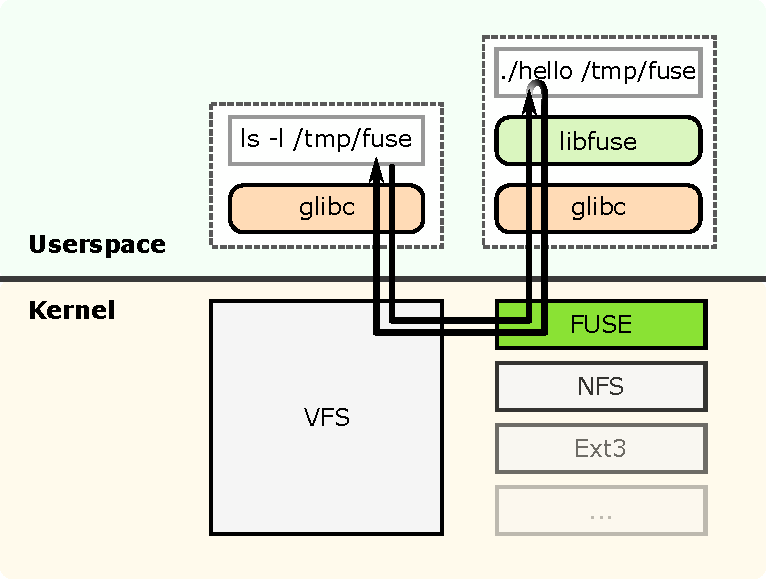
\includegraphics[width=\linewidth]{img/fuse_diagram}
    \caption{FUSE flow-chart diagram}\label{fig:fuse-diagram}
\end{figure}

FUSE has gained widespread adoption due to its ease of use and modularity.
Many popular file systems have been implemented using FUSE, such as SSHFS, GlusterFS, S3FS and NTFS-3G, among others.
These implementations demonstrate the versatility and robustness of the FUSE framework in handling a wide range of file system requirements.

Yet, FUSE is not without its limitations.
It is arguable whether it is the best choice for a C++ implementation, as it is written in C, but more on that later.
Another complication is its probability.
Fortunately, even though FUSE was initially designed for Linux, variants are available for other platforms, ensuring cross-platform compatibility:

\begin{itemize}
    \item \textbf{Linux}: libfuse - The reference implementation of FUSE~\cite{libfuse}.
    \item \textbf{macOS}: FUSE for macOS - A macOS port of FUSE~\cite{osxfuse}.
    \item \textbf{Windows}: WinFsp - A Windows File System Proxy that provides FUSE-compatible functionality~\cite{winfsp}.
\end{itemize}

Considering the advantages of user space development and the availability of FUSE for multiple platforms, FUSE is my preferred choice for implementing the proposed VFS\@.
This approach enables the development of a cross-platform VFS with versioning and encryption capabilities while avoiding the complexity of kernel driver development.
Still, several other libraries will need to be employed to address various aspects of the project.

\subsection{Encryption}\label{subsec:encryption-analysis}

Initially, Crypto++~\cite{crypto_pp} was considered for integration into the custom VFS, given its comprehensive open-source C++ class library covering a wide array of cryptographic schemes, such as encryption, hashing, and authentication algorithms.
Utilizing Crypto++ would provide file-level encryption, effectively safeguarding the security and privacy of the data stored within the VFS\@.

However, the implementation of Crypto++ led to various issues, primarily complicating the build process.
As a result, I decided to switch to libsodium~\cite{libsodium}, a more user-friendly alternative.
This modern, easy-to-use software library offers a robust selection of encryption, decryption, and cryptographic functions while maintaining a focus on simplicity and efficiency.
By incorporating libsodium, the custom VFS can achieve the desired level of data protection without incurring the complexities associated with Crypto++.

\subsection{Testing}\label{subsec:gtest}

Google Test~\cite{google_test}, commonly referred to as gtest, is a widely-used and adaptable C++ testing framework developed by Google.
This library enables efficient testing of individual components and the overall functionality of the custom VFS\@.
By employing gtest, the quality, reliability, and performance of the custom VFS can be evaluated, guaranteeing that it fulfills the requirements and expectations outlined in this thesis.

\subsection{Options parsing}\label{subsec:options-parsing}

The Boost Program Options library~\cite{boost_program_options} is a C++ library used for option parsing, which makes it easy to parse command-line options and arguments.
This library has been utilized for the custom VFS to handle different command-line options effectively, including setting the mount point, enabling or disabling debugging mode, and so on.

The Boost Program Options library has various features, such as automatic generation of help messages, support for positional arguments, and other abilities to handle advanced scenarios, such as parsing configuration files, environment variables, and even options passed through a graphical user interface.

I must also note that the Boost Program Options library has been used not only for the main VFS application but also for the supporting tools.